\chapter{Grundlagen}\label{ch:grundl}



\sectionDM{Spielprinzip von Josie - A Jelly's Journey}
\gamename  erinnert an eine erweiterte Version des Spieleklassikers Super Mario World.
In der Theorie sollte es mehrere Spielabschnitte geben, jedoch wurde aus zeitlichen Gründen nur ein Abschnitt implementiert. Ein Spielabschnitt besteht aus drei Jump and Run Levels und einem Boss Kampf Level. 

\paragraph{Jump and Run Level:}
Der Spieler versucht ohne Zeiteinschränkung das Level abzuschließen und dabei so viele Münzen wie möglich zu sammeln. Bei einem perfekten Lauf \textbf{kann} man alle Münzen einsammeln, einige davon sind allerding so plaziert dass sie nur schwer zu erreichen sind.
Dem Spieler stehen die Steuerungsfunktionen "'Stoppen"', "'Schrumpfen"' und "'Springen"' zur Verfügung. 
Dass Josie von selbst in einer festgelegten Geschwindigkeit läuft, führt zu einer gewissen Schwierigkeit des Spiels und macht Steuerungsfunktionen für "'Links"' und "'Rechts"' überflüssig.

\paragraph{Boss Level:}



\sectionTL{Einrichtung des verwendeten Frameworks}\label{sec:2_Framework}
Als die grobe Idee für das Spiel feststand, mussten wir uns für eine GameEngine entscheiden. Zur Auswahl standen unter anderem die AndEngine, Unity und Cocos2d-x. Nach ausreichender Recherche über die Funktionalitäten der verschiedenen Engines haben wir uns einstimmig für Cocos2d-x entschieden. Cocos2d-x untestützt drei Programmiersprachen, C++, JavaSkript und Lua. Hier haben wir C++ gewählt, da wir im laufe unseres Studiums eine Vorlesung über C++ gehört haben.
Die nächste Herausforderung war die Einrichtung von Cocos2d-x. Da wir drei verschiedene Betriebssysteme(Win8, MacOSX, Ubuntu) benutzen, hatten wir geringe Kompatibilitätsprobleme.
Um Cocos2d-x einzurichten, werden folgende Pakete benötigt:

\begin{itemize}
\item Cocos2d-x Link - \url{http://www.cocos2d-x.org/download}
\item Android SDK - \url{http://developer.android.com/sdk/index.html}
\item Android NDK - \url{http://androids.zone/android-ndk/#.VBLHNPldWXY}
\item Apache Ant - \url{http://ant.apache.org/bindownload.cgi}
\item Python - \url{https://www.python.org/downloads/}
\item Eclipse – \url{https://eclipse.org/downloads/}
\end{itemize}

Nachdem die Pakete heruntergeladen und ausgepackt sind, verschiebt man diese in den selben Ordner. Apache Ant und Python müssen installiert werden. Bei Python muss darauf geachtet werden das es sich um Version 2.x handelt. Unter Ubuntu muss Python nicht installiert werden, da dies schon in den Paketquellen vorhanden ist. 
Hat man die zwei Programme installiert öffnet man den Cocos2d-x Ordner und startet die setup.py Datei (über das Terminal). Daraufhin öffnet sich ein Terminalfenster in dem die Umgebungsvariablen angepasst werden, dies bedeutet man wird nach den Pfaden von der Android SDK/NDK, Apache Ant und Python gefragt. Entweder man gibt diese per Hand ein oder zieht die jeweiligen Ordner in das Terminalfenster. 



\sectionTL{Verwendete IDE und benötigte Plug-Ins}\label{sec:2_IDE}

Nachdem die Umgebungsvariablen eingetragen sind, muss das Android Developer Tool Plugin für Eclipse installiert werden. Hat man das erledigt öffnet man den im Plugin enthaltenen Android SDK-Manager und lädt sich hier nochmal die passende API herunter. In unserem Fall war das die API für Androidversion 4.4.2(API 19). 
Ist dieser Schritt geschafft, wird es Zeit das erste Projekt zu erstellen.
Hierzu öffnet man einen Terminal und wechselt in das Verzeichnis in dem auch der Cocos2d-x Ordner liegt. Hier gibt man folgenden Befehl ein:
	
\begin{lstlisting}[style=singleline]
	$cocos new MyGame -p com.MyCompany.MyGame -l cpp -d ~/MyCompany
\end{lstlisting}
		
\begin{itemize}
\item MyGame gibt den Namen des Projekts an
\item com.MyCompany.MyGame ist der Paketname für Android
\item cpp steht für die Programmiersprache. cpp für C++ und lua für Lua
\item ~/MyCompany gibt das Verzeichnis an in dem das Projekt gespeichert wird 
\end{itemize}

Der somit erstelle Ordner wird ins Git-Repository hochgeladen. 
Nun öffnet man wieder Eclipse und importiert das Git-Repository sowie die Cocos2d-x Bibliotheken. 

	Git-Repository: Eclipse → File → Import... → Git → 'Projects from Git'

Hier wählt man das vorher erstellte Projekt im Git-Repository aus.

	Cocos2d-x Bibliotheken: Eclipse → Import... → Android → 'Existing Android Code into 	Workspace'

Hier dirigiert man in das Verzeichnis in dem der Cocos2d-x Ordner liegt und wählt diesen komplett aus. Im nachfolgenden Fenster wählt man alle vorgeschlagenen Punkte ab bis auf libcocos2dx Nachdem beide 'Projekte' importiert wurden, wählt man sein Projekt aus dem Git-Repository aus und wechselt in die Einstellungen. Unter dem Reiter 'Android' ist darauf zu achten, dass als Library das Projekt libcocos2dx ausgewählt ist. Ist es nicht in der Liste enthalten, fügt man es mit 'Add' hinzu. 

Es ist darauf zu achten, dass sich alle Ordner inkl. dem Git-Repository in einem Ordner befinden.

Zu guter Letzt, öffnet man die AndroidManifest.xml in Eclipse aus und ändert hier den Wert auf die Entsprechende API.
\begin{lstlisting}[style=singleline]
	<uses-sdk android:minSdkVersion="19"
			  android:targetSdkVersion="19"/>
\end{lstlisting}
	

Nun kann man anfangen zu arbeiten! 



\sectionTL{Szenenprinzip}\label{sec:2_Szenenprinzip}
Eine Szene ist im Grunde genommen nichts anderes als ein Container, welcher  Sprites, Labels, Nodes und andere Objekte beinhaltet die ein Spiel benötigt. Eine Szene ist für die laufende Spiellogik und Darstellung des Inhaltes auf einer 'per-frame basis' verantwortlich. Es wird mindestens eine Szene benötigt damit man das Spiel starten kann. Man kann beliebig viele Szenen-Objekte in einem Spiel verwenden und leicht zwischen diesen überleiten. Der Vorteil von Szenen liegt darin, dass man nicht jedes Objekt einzeln laden muss. An eine Szene lassen sich diverse Sprites, Labels und Nodes mit der von Cocos2d-x gegebenen Funktion addChild() anhängen(siehe Abbildung \ref{fig:szenengraph}). Sobald das Szenen-Objekt geladen wird, werden die angefügten Kinder mitgeladen. Dies spart Zeit und entlastet den Speicher.

\begin{figure}[H]
  \centering
  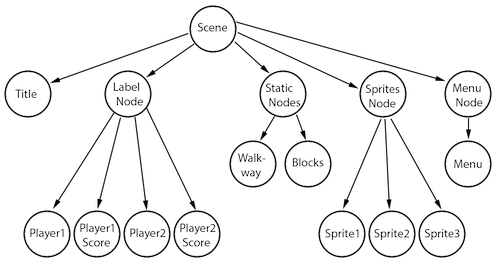
\includegraphics[width=12cm]{resources/scenegraph}
  \caption{Szenengraph}
  \label{fig:szenengraph} 
\end{figure}


\subsection{Szenenfunktionen von cocos2d}

Cocos bietet Funktionen an um Szenen zu erstellen und zwischen diesen zu wechseln. Um einen Szenenwechsel durchzufüren, muss zuerst eine Szene erstellt werden.

\begin{lstlisting}[style=singleline]
	Szene* Cutscene = Szene::create();
\end{lstlisting}


Dies erstellt ein Objekt des Typ Szene mit dem Namen Cutscene.
Im Laufe des Spiels ist es  notwendig zwischen den verschiedenen Szenen zu wechseln. Dies wird deutlich, wenn man z.B. ein neues Spiel starten oder ein anderes Level auswählen möchte. Hierzu stellt Cocos2d-x verschiedene Funktionen bereit eine Szene zu wechseln.

\begin{itemize}
\item replaceScene() ersetzt eine Szene vollständig durch eine Andere
\item pushScene() unterbricht die Ausführung der aktuellen Szene und verschiebt diese auf den Stack. Der Stack ist eine Art Warteschlange welche nach dem 'Last in, First out – Prinzip', dort wartet die Szene auf weitere Anweißungen. Diese Funktion darf nur aufgerufen werden, wenn bereits eine Szene aktiv ist.
\item popScene() wiederum ersetzt die aktuelle Szene und löscht diese komplett. Diese Funktion darf nur aufgerufen werden, wenn bereits eine Szene aktiv ist.
\end{itemize}



\sectionDG{Spriteprinzip}\label{sec:2_Spriteprinzip}
Allgemein betrachtet kann man sagen, dass ein Sprite(engl. Kobold, Geistwesen) ein Grafikobjekt ist, welches über den Hintergrund gelegt wird und von der Grafikhardware platziert wird. 
Der Name rührt daher, dass ein Sprite auf dem Bildschirm umherspäht und im Grafikspeicher nicht zu finden ist. Heutzutage bezeichnet der Begriff “Sprite” jedoch alle Objekte die so aussehen wie ein solches Grafikobjekt, jedoch eigentlich von einer Software erzeugt werden und im Grafikspeicher vorliegen. 
Solche softwareerzeugten Sprites sind streng genommen “Shapes”, für deren Erzeugung überwiegend die CPU zuständig ist.
 
Für Computerspiele sind mit Sprites einige Vereinfachungen verbunden. So werden zum Beispiel in vielen 2D Jump and Run Spielen so genannte Tiles oder auch Kachelgrafiken verwendet, welche ebenfalls kleine Grafikelemente sind die zusammengesetzt eine größere Grafik ergeben. Ihr Anwendungsbereich findet sich unter anderem im Aufbau eines Levels, wobei aus ihnen die Spielwelt zusammengesetzt wird.

\subsection{cocos2d Spriteprinzip}
In der von uns verwendeten Gameengine cocos2d, ist ein Sprite ein “Bild”, welches durch Veränderung seiner Werte manipuliert werden kann. Es gibt verschiedene Wege ein Sprite zu erstellen, je nach dem wozu es benutzt werden soll. Bezüglich Dateiformaten werden von cocos2d PNG, JPEG, TIFF etc. unterstützt. Wir haben uns für das Dateiformat PNG entschieden, da es eine gute Komprimierung, gute Qualität, Darstellung von Halbtransparenzen, also 50\% Deckraft, vorweist und außerdem ein sehr weit verbreiteter Datentyp ist.

Es gibt unterschiedliche Methoden ein Sprite zu erstellen. Eine Möglichkeit ist das Sprite aus einem Bild zu laden, wobei das in cocos2d erstellte Sprite Objekt die selben Abmessungen wie das benutzte Bild vorweist. 

\begin{lstlisting}[style=singleline]
Sprite* mySprite = Sprite::create("mysprite.png");
\end{lstlisting}

Eine weitere Methode ist das Erschaffen eines Sprites durch Angabe eines Ausschnittes des benutzten Bildes. Dabei wird im Erstellungsprozess ein so genanntes \texttt{Rect} angegeben, welches die Position als auch die Dimension auf dem Bildschirm darstellt. 

\begin{lstlisting}[style=singleline]
Sprite* mySprite = Sprite::create("mysprite.png", Rect(0,0,40,40));
\end{lstlisting}

Die Möglichkeit ein Sprite aus einem Spritesheet zu erstellen ist besonders empfehlenswert. Ein Spritesheet ist eine Bilddatei in der mehrere Sprites beliebig aneinander gereiht gespeichert werden können. Dies birgt den Vorteil, dass nur eine Datei geladen werden muss anstatt viele einzelne Bilder, was die Ladezeiten erheblich verringert und zudem eine Speicherreduktion mit sich bringt. Außerdem reduzieren diese die Aufrufe an OpenGL ES etwas zu zeichnen und zu rendern. Beim erstmaligen verwenden eines Spritesheets, wird dieses in den \cocosclass{SpriteFrameCache} geladen. Dies ist eine Klasse, welche ein \cocosclass{SpriteFrame} Objekt, für zukünftigen Schnellzugriff speichert. SpriteFrame-Objekte beinhalten den Bildnamen des Sprites und ein \texttt{Rect} um die Größe des Sprites zu spezifizieren. Aus dem SpriteFrameCache, in welchem das Spritesheet geladen wurde, kann nun ein Sprite erstellt werden.
Spritesheets stellen in unserem Projekt speziell für Animationen und die Umgebung der Spielwelt eine optimale Lösung dar. 



\subsection{Möglichkeiten Sprites zu manipuliern}
Der Ankerpunkt eines Sprites ist ein Punkt, welcher zur Orientierung bei der Positionsbestimmung eines Sprites dienen soll. Der Ankerpunkt benutzt ein Koordinaten System das von 0 bis 1 geht, wobei \texttt{0,0} unten links und \texttt{1,1} oben rechts vom Sprite ist.

\begin{lstlisting}[style=singleline]
Sprite* mySprite->setAnchorPoint(0,0); // (0,1), (1,0), (0.5,0.5)
\end{lstlisting}

\begin{figure}[H]
  \centering
  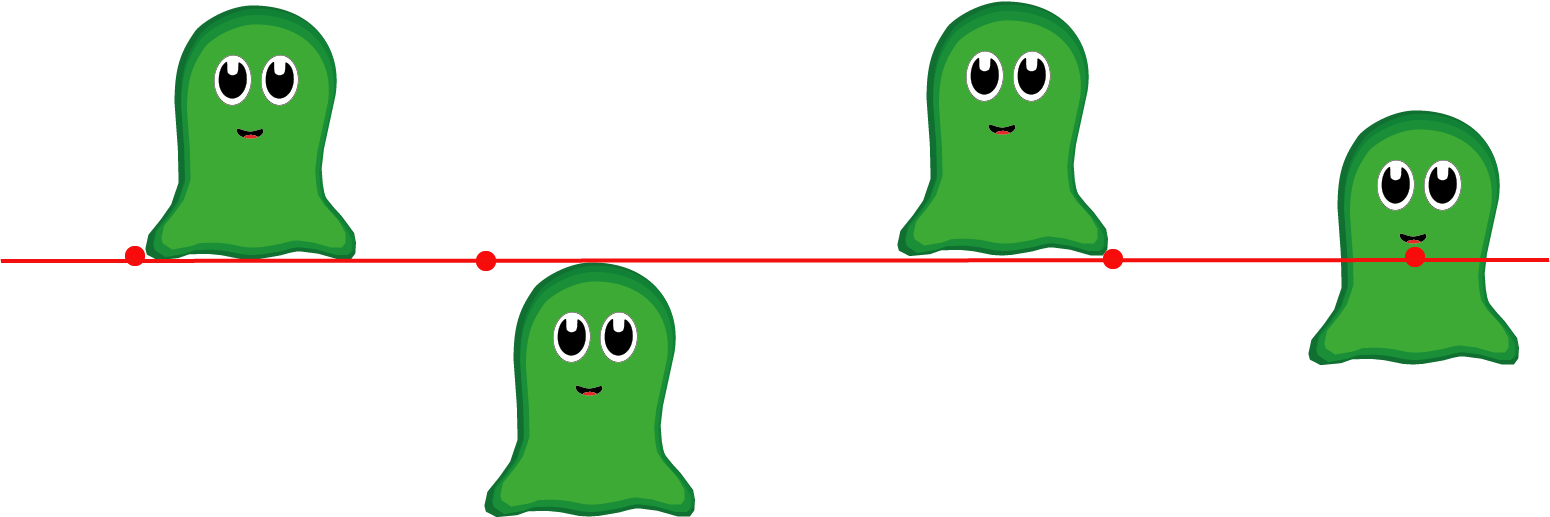
\includegraphics[width=10cm]{resources/josiedoku3}
  \caption{Plazierung von Josie bei verschiedenen Ankerpunkten (rot)}
  \label{fig:josie_ancherpoint} 
\end{figure}

Möglichkeiten ein Sprite zu manipulieren sind unter anderem Skalieren, Rotieren und Verzerren. Weiterhin kann man die Farbe und Sichtbarkeit eines Sprites verändern. Die in unserem Projekt am häufigsten verwendete Manipulationsmethode ist das Skalieren. Sie ermöglicht es die Größe eines Sprites beliebig zu verändern.

\begin{figure}[H]
 \centering
  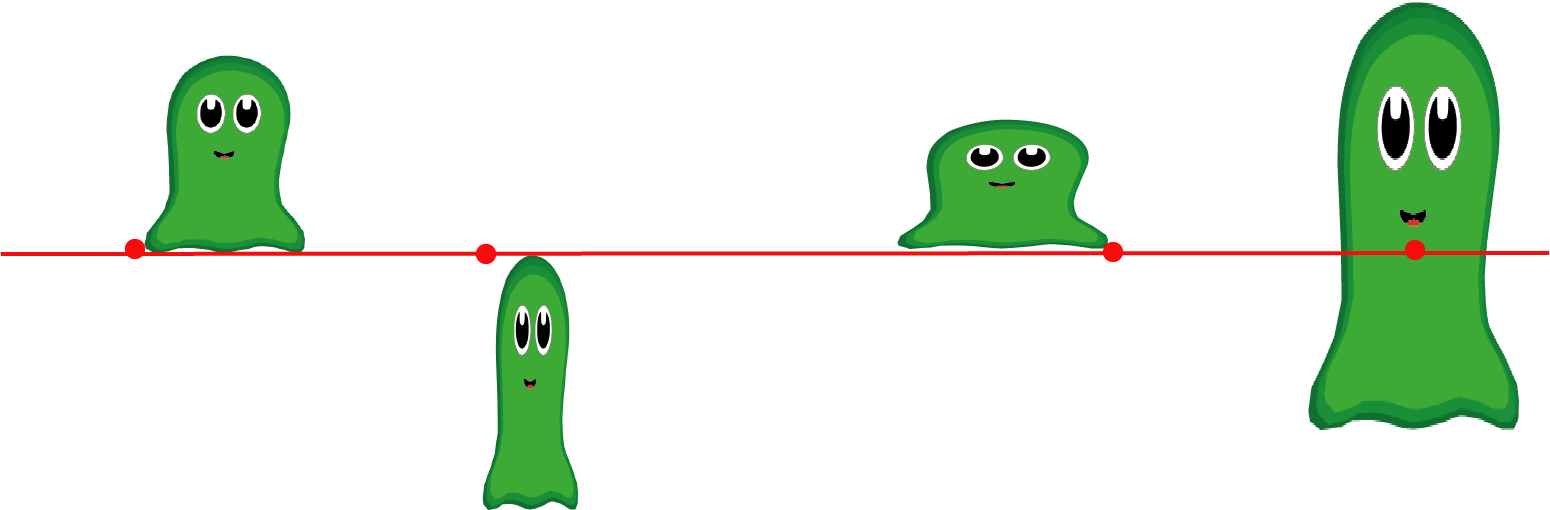
\includegraphics[width=10cm]{resources/josiedoku4}
  \caption{Josie nach dem Skalieren}
  \label{fig:josie_scale} 
\end{figure}



\sectionDG{Animationsprinzip}\label{sec:2_Animationsprinzip}

\subsection{Allgemeines und cocos2d Spriteprinzip}
Im Verlauf unseres Projektes wurden verschiedenste Animationen benutzt. Im folgenden soll ein kurzer Einblick in das Prinzip der Animationen in cocos2d, als auch allgemein gewährt werden. Einfach gesagt sind Animationen nichts weiter als eine sehr schnell abgespielte Aneinanderreihung von Bildern. In der Computergrafik oder bei Computerspielen werden diese verwendet um den Spielecharakter zum Leben zu erwecken und das Spiel dynamischer zu machen. Ohne sie wären Spiele nicht grafisch darstellbar.

In cocos2d werden solche Animationen durch \cocosclass{Action} Objekte realisiert. Diese haben die Fähigkeit die Werte von \cocosclass{Node} Objekte, in Echtzeit zu transformieren. Dazu zählen ebenfalls Instanzen der Klassen die von einem solchen Objekt erben. Werte eines Nodes, die verändert werden können sind z.b. die Sichtbarkeit, Farbe, Position oder auch die Größe des Nodes. Zum Beispiel kann ein Sprite von einer Position zur anderen bewegt werden.

Grundsätzlich können zwei Versionen von Actions unterschieden werden, diese sind By und To. Wobei Letztere absolut sind und im Gegensatz zu By Actions d.h. sie berücksichtigen die aktuelle Position des Node nicht. Ein mögliches Beispiel für eine MoveTo Animation soll im folgenden kurz beschrieben werden. Man erstellt ein MoveBy Objekt mit einer Angabe über die Dauer der Animation in Sekunden sowie ein Vektor der die Ziel Koordinaten auf der X als auch die der Y Achse beinhaltet. Anschließend wird dieses Objekt auf einem Node z.b. ein Sprite durch die Methode \textbf{runAction()} ausgeführt. 

\begin{figure}[H]
 \centering
  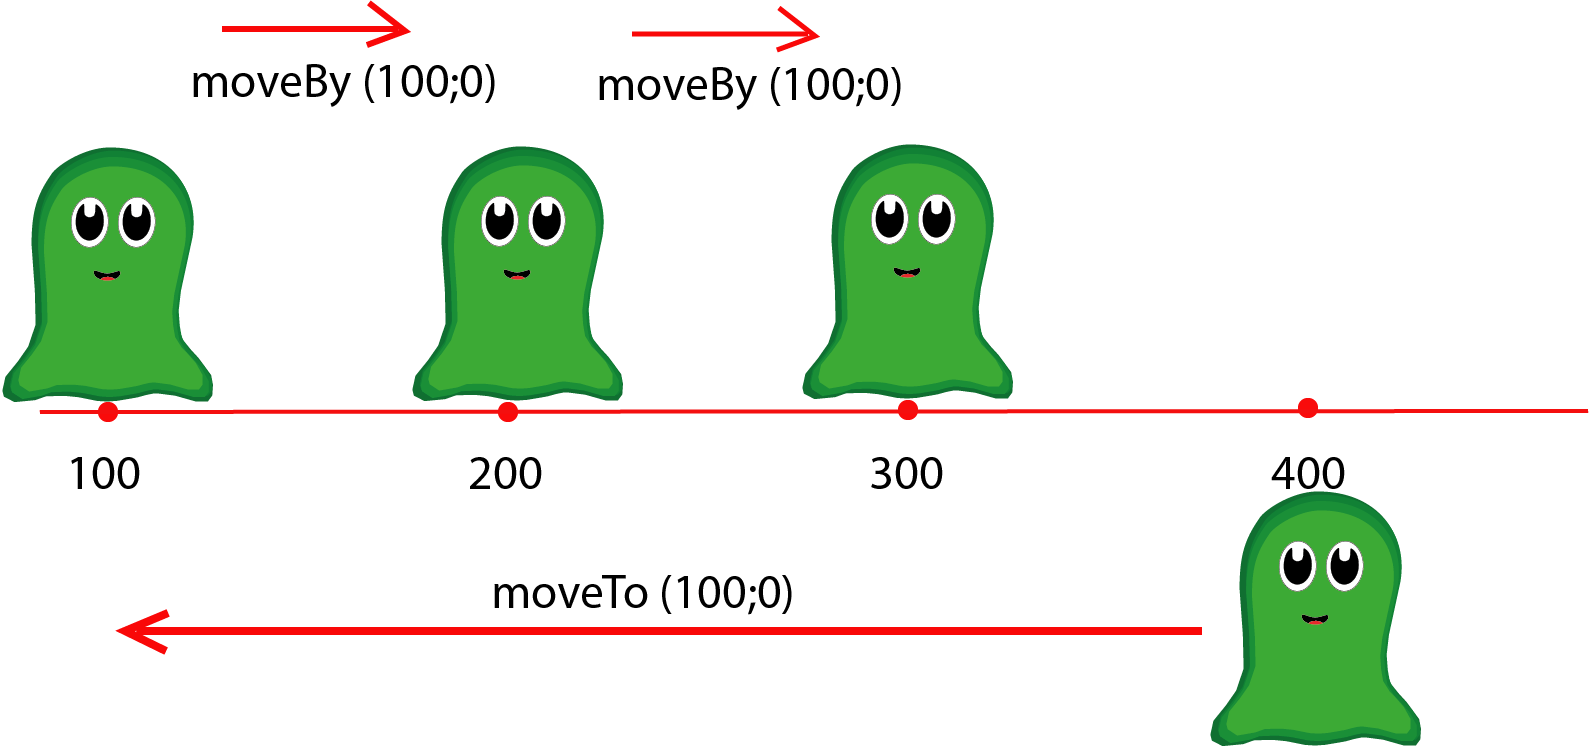
\includegraphics[width=10cm]{resources/josiedoku6}
  \caption{Unterschied zwischen MoveBy und MoveTo}
  \label{fig:josiemoveByTo} 
\end{figure}

Die von cocos2d bereitgestellten Funktionen zur Veränderung von Nodes sind Move, Rotate, Scale, Fade In/Out und Tint.

\begin{figure}[H]
 \centering
  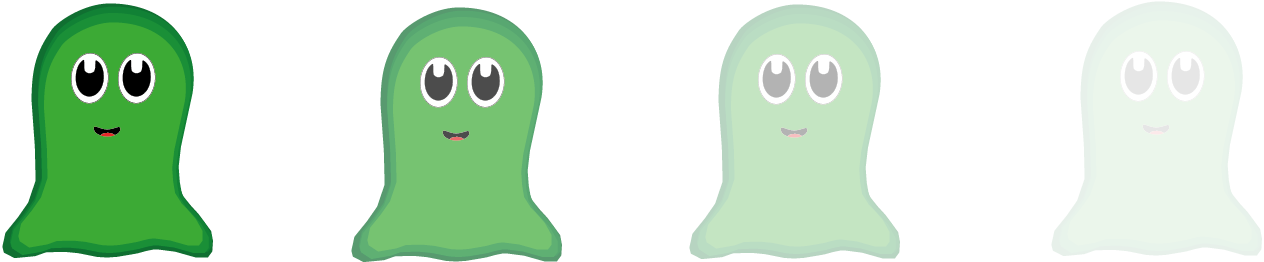
\includegraphics[width=10cm]{resources/josiedoku5}
  \caption{Beispiel für Fade In/Out bei Josie}
  \label{fig:fade} 
\end{figure}


\subsection{Animate und Sequenze}
Im vorangegangenen Abschnitt wurden ein Überblick einiger cocos2d bereitgestellter Animationen geschaffen. Im Verlauf eines Spieleprojektes wäre es jedoch sinnvoll eigene Animationen erstellen zu können. Eine Möglichkeit eigene Animationen zu erstellen wie zum Beispiel eine Art simples Daumenkino, bietet die Klasse \cocosclass{Animate}. Ein Animate enthält eine Animation bzw. wird aus dieser Erstellt. Animations sind Container welche durch die SpriteFrame Verzögerungszeit zwischen den Frames als auch die Dauer der Action bestimmt werden. Wenn ein Animate Objekt ausgeführt wird, werden bestimmte Frames auf dem Display durch die in dem Animate enthaltenen, ersetzt. So kann zum Beispiel ein SpriteFrame durch ein Set von SpriteFrames ersetzt werden.

Um Komplexe Abläufe von Animationen zu definieren ist es sinnvoll eine Klasse wie \cocosclass{Sequence} zu benutzen. Die Instanz einer Sequence ermöglicht es verschiedene Action, Function und sogar Sequence Objekte hintereinander zu reihen und in einem Sequence-Objekt zusammenzufassen. So können Abläufe von Animationen zusammengefasst werden.

\begin{figure}[H]
 \centering
  
\includegraphics[width=10cm]{resources/sequence}
  \caption{Beispiel für Sequenzen}
  \label{fig:sequence} 
\end{figure}

Ein Zusammenspiel von Grundfunktionen und Sequenzen fand in unserem Projekt bei den Angriffspattern des Boss Gegners Anwendung. Hierbei war ein Problem, dass sich bei zu kurzem Puffer und zu langen Aktionszeiten die einzelnen Aktionen vermischen.

Eine weitere Vereinfachung durch cocos2d bietet die Reverse Methode. Diese dient dazu Animationen rückwärts ablaufen zu lassen. Diese ist in unserem Projekt unter anderem bei der Sprung Animation zum Einsatz gekommen.


\subsection{Spritesheet}

Eine häufige Methode zur Spriteerstellung ist es das Spritesheet bei der Erzeugung in den Cache zu laden. 
Hierzu benötigt man nicht nur das Spritesheet sondern auch eine beschreibende “.plist” Datei, die eine Zuweisung von SpriteFrame zu Bildern und deren Position im Spritesheet enthält. Nun kann man einerseits durch ein Zusammenspiel zwischen Spritesheet und .plist Datei die Animation bzw. den Ablauf im eigenen Programm definieren. Hierbei werden die SpriteFrame und die .plist Datei geladen, um im Anschluss die SpriteFrames in der .plist Datei mit den Sprites aus dem Spritesheet zu koppeln. Andererseits kann man den Ablauf einer Animation in der .plist Datei festlegen und im Anschluss die fertige Animation laden.

Wir entschieden uns für die Spritesheet .plist Methode, da wir ebenfalls bei der Realisierung des Levels mit Spritesheets arbeiteten und die Arbeit mit diesen daher kennen. Bei der Suche nach einem Programm für die “Datei Methode” fanden wir weiterhin nur schlechte Tutorials.



\sectionOG{Datenkommunikation}

\subsection{Callbackprinzip}\label{sec:2_Callbackprinzip}
In vielen Teilen des Spieles wird \textbf{CC\textunderscore CALLBACK\textunderscore 0()} verwendet - unter anderem für Menü-Buttons. Ein Callback wird verwendet um einer Funktion, eine andere Funktion als Parameter zu übergeben. Im Besonderen wenn vorher nicht klar ist, wann diese Funktion ausgeführt wird (bsp. Klick auf einen Button). Genau genommen ist es nur ein Makro für die C\texttt{++} Funktion \textbf{std::bind}. Anstatt der Null könnte man auch eine Eins angeben um zusätzlich den Sender als Parameter zu übergeben.

Hier sei noch kurz das \textbf{CallFuncN} erwähnt. Das Callback wird in eine \cocosclass{Action} gekapselt, um die Funktion innerhalb einer Animations Sequenz auszuführen (S: \pageref{lst:CallFuncN}).


\subsection{Observer Pattern}

Für die Spielersteuerung (Kapitel \ref{sec:4_SpielerSteuerung}) wird ein Observer Pattern verwendet. Auch hier ist der Hintergrund die asynchrone Abarbeitung von Benutzer Ereignissen. Im Unterschied zum Callback geht es beim Observer immer um mindestens zwei Objekte, dem der die Nachricht sendet und dem der sie empfängt. Es können aber sowohl mehrere Empfänger (bsp. Radio), als auch mehrere Sender (bsp. Tempomat und Fahrer beeinflussen die Geschwindigkeit) beteiligt sein.

\begin{figure}[H]
 \centering
  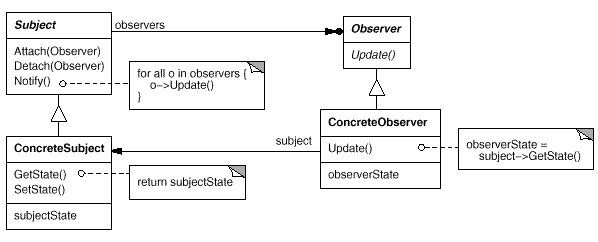
\includegraphics[width=15cm]{resources/observer_pattern}
  \caption{Observer Patter aus \cite[Design Patterns]{gamma2011patterns}}
  \label{fig:observer_pattern} 
\end{figure}

Der Empfänger trägt sich selbst in eine Liste von Empfängern für ein bestimmtes Event/Namen ein und meldet somit sein Interesse für das Ereignis. Bei Eintreffen des Ereignisses geht der Sender die Liste der Empfänger durch und informiert jeden über das neue Ereignis.



\sectionJK{Tilemaps}\label{sec:2_Tilemaps}

Tilemaps  sind spezielle Dateiformate, welche die Landschaft im Spiel, sowie die dazugehörigen Daten beschreiben. Charakteristisch für sie ist eine Untergliederung der Spielwelt in rechteckige oder Hexagon-förmige Felder (Wobei in seltenen Fällen auch andere Formen verwendet werden). Durch Tilemaps wird für diese Schachbrettartige Landschaft die grafische Darstellung sowie darüber hinaus Eigenschaften der Umwelt (Kollisionen, Spawn-Punkte usw.) festgelegt.

\subsection{Vorteile der Tilemap}
Als die Videospiel-Branche noch in den Kinderschuhen steckte, mussten Entwickler vor allem eines berücksichtigen: Der nur sehr begrenzt verfügbare RAM musste möglichst effektiv genutzt werden. Eine Idee um diesen Speicher effizienter zu nutzen war die Tilemap. Landschaften in Spielen sind oft in einem Stil gehalten – d.h. oft wiederholen sich Teile der Umgebung wieder und wieder. Anstatt also die gesamte Spielwelt in großen Bilddateien zu speichern die viel RAM beanspruchen, werden stattdessen nur die Komponenten aus denen die Umwelt besteht, in einer kleineren Datei/vielen kleinen Dateien gespeichert. Die Tilemap beschreibt dann, wie diese Komponenten angeordnet werden müssen, um die Welt zu erschaffen.

Auch bei der Gestaltung der Level bieten Tilemaps einen großen Vorteil. Da man sich die Welt quasi zusammenpuzzelt, können Änderungen an Teilen der Landschaft leicht durchgeführt werden, ohne die gesamte Welt neu erschaffen zu müssen. Je nachdem wie genau das verwendete Tilemap-Format aufgebaut ist, kann theoretisch sogar ein Texteditor verwendet werden um schnell ein Level aus bestehenden Komponenten zu gestalten. Für gewöhnlich benutzt man jedoch Tools, die den Prozess visuell unterstützen. Level-Designer können sich so vollständig auf das Gestalten der Spielwelt konzentrieren, ohne sich Sorgen um den Code zu machen.

\subsection{Funktionsweise von Tilemaps}
Allgemein benötigt die Tilemap zwei Dinge um eine Umgebung im Spiel vollständig beschreiben zu können. Einerseits den "'Map-part"' - ein 2-dimensionales Feld, welches Verweise auf den Inhalt der jeweiligen Kachelkoordinate beinhaltet. Andererseits wird noch ein Tileset benötigt. Die einzelnen Tiles sind dabei Objekte, die das Aussehen und die Eigenschaften beschreiben, welche einer Kachel zugewiesen werden können.

Eigenschaften sind frei wählbar, da sie in Form von Key-Value-Pairs gespeichert werden, die im Code des Spiels abgefragt werden können. Häufig genutzte Eigenschaften sind beispielsweise Kollisionen, die Auswirkungen des Felds auf den Spielercharakter usw. Auch Spawn-Positionen für Objekte in der Spielwelt können Eigenschaften von Kacheln sein, wobei dafür in vielen Fällen auch andere Funktionen des Tilemap-Formats genutzt werden könenn (diese sind jedoch nicht bei allen Formaten vorhanden). 

Neben den Eigenschaften verweist jedes Tile auch auf die Grafik, die angezeigt werden soll wenn das Tile im Spiel dargestellt wird. Dafür wird ein Spritesheet verwendet, dessen einzelne Sprites in der Größe identisch mit der Kachelgröße der Tilemap sind.
Die meisten Tile-Engines bieten noch weitere Features, wodurch die Tilemaps noch mächtiger werden. Beispielsweise ist es heute nahezu Standard, dass Tilemaps „Layer“ unterstützen. Durch den Aufbau aus verschiedenen Ebenen können so Tiles miteinander kombiniert werden. Dies geschieht sowohl grafisch - indem die Kacheln hintereinander Dargestellt werden -  als auch auf Ebene der Eigenschaften. Oft wird eine Eigenschaftsebene angelegt (sie ist später im Spiel für gewöhnlich unsichtbar), auf der Tiles platziert werden die jeweils eine Eigenschaft bzw. eine Kombination aus Eigenschaften repräsentieren. Indem man die Eigenschaften von der Grafischen Ebene löst, bietet man dem Designer der Level einen größeren Grad an Freiheit. Sinnvoll ist das jedoch bloß, wenn Kacheln mit derselben Grafik nicht zwangsweise auch dieselben Eigenschaften haben sollen. 

Ein weiteres Feature, das nicht immer vorhanden ist, sind Objekte. Geometrische Formen, die unabhängig vom Kachelmuster sind erlauben es dem Entwickler Punkte und Bereiche in der Tilemap festzulegen, die abseits des regelmäßigen Rasters liegen. Genau wie Tiles, könen auch sie mit Eigenschaften versehen werden.

\subsection{Tilemaps in cocos2d}
Cocos2d unterstützt ein einziges Tilemap-Format: TMX (Tile Map XML). In diesem Format kann eine Tilemap mit beliebig vielen Ebenen gespeichert werden. Jede Ebene kann dabei nur ein Tileset verwenden, das gleiche Tileset kann jedoch auf verschiedenen Ebenen genutzt werden. TMX unterstützt die beiden häufigsten Formen von Tiles: Rechtecke und Hexagone. 
Zusätzlich zu den Kachelebenen können auch Objektebenen erstellt werden. Hier können die zuvor erwähnten Objekte platziert werden, um auch unabhängig vom festgelegten Raster arbeiten zu können (Tiles können hier jedoch nicht platziert werden).
Dateien im TMX Format werden mit dem Tiled Mapeditor erstellt. In der Online Dokumentation des Editors findet man auch eine umfangreiche Erklärung über den Aufbau des TMX-Formats \cite{TiledDocFormat}.

Cocos2d liefert durch die Klassen des Tilemap Moduls Funktionen, um den Umgang mit Tilemaps im Programmcode einfacher zu gestalten. Im Folgenden soll kurz gezeigt werden, wie man eine Tilemap im Spiel anzeigt und sich Informationen über diese beziehen kann bzw. wie man diese bearbeitet.

Um eine Tilemap anzuzeigen muss lediglich ein Objekt vom Typ \cocosclass{TMXTiledMap} erstellt werden und als Child in der aktuellen Szene angefügt werden. In unserem Code ist der Prozess über verschiedene Funktionen verteilt, weshalb hier nur ein einfaches allgemeines Beispiel gezeigt wird:

\begin{lstlisting}[style=singleline]
TMXTiledMap map = create("Path/Map.tmx");
currentScene.addChild(map);
\end{lstlisting}

Um einzelne Ebenen in Form von TMXLayer Objekten abzufragen nutzt man folgende Funktion:

\begin{lstlisting}[style=singleline]
TMXLayer* ebene = map.getLayer("NameDerEbene");
\end{lstlisting}

Ähnlich erhält man ein Tile Objekt mit:

\begin{lstlisting}[style=singleline]
Sprite* kachel = ebene->tileAt(Vec2(x, y));
\end{lstlisting}

X und y sind hier die Koordinaten des Felds auf der Ebene.
Um zu bestimmen welches Tile an einer Position liegt (und nicht bloß den Sprite zu erhalten) benutzt man:

\begin{lstlisting}[style=singleline]
unsigned int gid = ebene->getTileGIDAt(Vec2(x,y));
\end{lstlisting}

Anhand der GID kann man auch zur Laufzeit ein Tile an einer beliebigen Position platzieren bzw. ersetzen. Dabei erhält die Kachel selbstverständlich auch alle Eigenschaften der gewählten GID	

\begin{lstlisting}[style=singleline]
ebene->setTileGID(gid, Vec2(x,y));
\end{lstlisting}

Die Attribute eines Feldes erhält man ebenfalls über einen simplen Funktionsaufruf:

\begin{lstlisting}[style=singleline]
Value werte = map.getPropertiesForGID(gid);
ValueMap eigenschaften = werte.asValueMap();
\end{lstlisting}

Nun kann man die Eigenschaften über die vergebenen Namen aus der ValueMap ermitteln. Oft ist dies jedoch nicht nötig, da man eventuell bereits weiß, welche GID über welche Eigenschaften verfügt.

Cocos2d stellt noch hunderte weitere Funktionen bereit um Tilemaps zu handhaben, jedoch reichen die hier genannten aus, um mit den Kacheln der Tilemap zu arbeiten. Objekte als Elemente der Tilemaps werden in diesem Projekt nicht verwendet, jedoch ist auch der Zugriff auf sie vollständig durch Getter und Setter abgedeckt.



\sectionDM{Musik und Sound-Effekte}\label{sec:2_Musik}
Jegliche Musik und Soundeffekte die in unserem Spiel \gamename zu hören sind wurden selbst geschrieben, aufgenommen und bearbeitet. Dazu gehören die
\textbf{Hintergrundmusik} im Hauptmenü, in der Levelauswahl, in den Jump and Run Levels und im Boss Kampf. Außerdem \textbf{Soundeffekte} für das Springen, Schrumpfen, Stoppen und Schießen, sowie das kaufen von Aufwertungen und das Treffen des Endgegners.



\subsection{Möglichkeiten der cocos2d-Engine zur Audioverarbeitung}
Cocos2d bietet mit der \cocosclass{SimpleAudioEngine} eine relative einfache Möglichkeit Audio\-dateien, sei es die Hintergrundmusik oder ein Sound--Effekt, zu laden, abzuspielen, zu pausieren und wieder zu entfernen/entladen. Hierzu ein kurzes Beispiel wie man auf einfache Art und Weise eine Audiodatei abspielt.

\begin{lstlisting}[style=singleline]
SimpleAudioEngine::getInstance()->playBackgroundMusic("song.mp3",true);
\end{lstlisting}

Auf die Implementierung und die Verwendung der \cocosclass{SimpleAudioEngine} innerhalb unseres Codes wird im Kapitel \ref{sec:4_Audiounit} genauer eingegangen. Vorweg sei gesagt dass wir alle Funktionalitäten welche die \cocosclass{SimpleAudioEngine} betreffen in eine eigene statische Klasse \josieclass{AudioUnit} ausgelagert haben.


\subsection{Monofonie/Stereofonie und verwendete Dateiformate}
Es ist möglich sowohl monofone als auch stereofone Audiodateien zu verwenden. Falls man möchte dass Sounds zum Beispiel aus bestimmten Richtungen kommen, um dem Spieler ein gewisses "'Mittendrin--Gefühl"' zu vermitteln, sollten die Audiodateien stereofon sein. Das ist allerdings erst richtig sinnvoll wenn das Spiel mit Kopfhörern oder mit Anschluss an ein Soundsystem gespielt wird. 

Im Fall von \gamename wurden sterefone Audiodateien ohne oder geringem Panning (mischen von einzelnen Instrumenten/Klängen nach links oder rechts) verwendet, da das Spiel hauptsächlich für mobile Geräte gedacht ist und diese meist nur über einen Lautsprecher verfügen. Zudem werden in der Realität Spiele auf mobilen Geräten meist ohne Ton oder Kopfhörer gespielt, sodass wir deshalb keinen speziellen Wert auf räumlichen Klang gelegt haben.

Es wurde auschließlich "'mp3"' als Format für Audiodateien verwendet, da dieses Dateiformat in Bezug auf cocos2d von den meisten Geräten unterstützt wird. Ein weiterer Vorteil von "'mp3"' gegenüber anderen Formaten wie "'wav"' ist die durch die verschiedenen Abtastraten entstehende Dateigröße, worauf hier allerdings nicht im Detail eingegangen wird. Dieser Dateigrößenunterschied ist im Bezug auf mobile Geräte ein sehr wichtiger Faktor.

%\newpage
\subsection{Audiobearbeitungsprogramme}
Auf dem Softwaremarkt gibt es unzählige Audiobearbeitungsprogramme. Wenn man sich mit dem Thema Audiobearbeitung noch nie beschäftigt hat, ist es sehr schwer eines zu finden das die nötigen Funktionen liefert um einen gutes Resultat zu erzielen. Zudem kosten die meisten guten Programme viel Geld. Im Folgenden soll eine Auflistung von einigen kostenplfichtigen und kostenlosen Programmen einen groben Überblick verschaffen. Bei den kostenpflichtigen Programmen ist die Preisspanne sehr groß, da es auch auf Version und Ausführung ankommt, deshalb sind an dieser Stelle auch keine Preise genannt.

\begin{itemize}
 \item Cubase (Steinberg, kostenpflichtig)
 \item Pro Tools (Avid, kostenpflichtig)
 \item Logic Pro (Apple, kostenpflichtig)
 \item Musik Maker (MAGIX, kostenpflichtig)
 \item Goldwave (Goldwave Inc., teilweise kostenlos)
 \item Audacity (AudacityTeam, kostenlos)
 \end{itemize} 

Bei \gamename wurde Logic Pro X von Apple verwendet. 

